\chapter{NLMaps Data Improvement}
\label{ch:nlmaps-improvement}

After training a character-based encoder-decoder model as described by
\textcite{staniek-2020} on the \nlmapstwo{} dataset, it quickly becomes apparent
that the \SI{93.8}{\%} performance on the test split is not reflected in the
model’s performance on new queries. In particular, the model is not robust
against unseen wordings of a query and it – more understandably – also fails for
unseen OSM tags. Figure~\ref{fig:nlmaps-v2-reality-check} shows typical errors
the model makes on NL queries from \nlmapsfour{}, which is
introduced in Section~\ref{sec:annotation}.

\begin{figure}[h]
  \centering
  \begin{subfigure}{\textwidth}
    \begin{minipage}{0.48\textwidth}
      \begin{lstlisting}[style=MyMRL,title={Gold MRL},basicstyle={\ttfamily\scriptsize}]
query(
  around(
    center(
      area(keyval('name','Westheim')),
      nwr(
        keyval('name','Martinskirche')
      )
    ),
    search(
      nwr(keyval('amenity','cafe'))
    ),
    maxdist(DIST_INTOWN)
  ),
  qtype(latlong)
)
      \end{lstlisting}
    \end{minipage}
    \hfill
    \begin{minipage}{0.48\textwidth}
      \begin{lstlisting}[style=MyMRL,title={System MRL},basicstyle={\ttfamily\scriptsize{}}]
query(
  around(
    center(
      area(keyval('name','Westheim')),
      nwr(
        keyval('name','Martinskirche')
      )
    ),
    search(
      nwr(keyval('amenity','cafe'))
    ),
    maxdist(DIST_INTOWN)
  ),
  (@\textcolor{red}{qtype(show:me)}@)
)
      \end{lstlisting}
    \end{minipage}
    \caption{\nl{Show me the cafes near Martinskirche in Westheim}}
    \label{fig:cafes-near-martinskirche}
  \end{subfigure}
  \begin{subfigure}{\textwidth}
    \begin{minipage}{0.48\textwidth}
      \begin{lstlisting}[style=MyMRL,title={Gold MRL},basicstyle={\ttfamily\scriptsize}]
query(
  around(
    center(
      nwr(keyval('name','Zenica'))
    ),
    search(
      nwr(keyval('natural','valley'))
    ),
    maxdist(DIST_OUTTOWN)
  ),
  qtype(least(topx(1)))
)
      \end{lstlisting}
    \end{minipage}
    \hfill
    \begin{minipage}{0.48\textwidth}
      \begin{lstlisting}[style=MyMRL,title={System MRL},basicstyle={\ttfamily\scriptsize{}}]
query(
  around(
    center(
      (@\textcolor{red}{area(keyval('name','Paris')),}@)
      nwr(keyval('name','Zenica'))
    ),
    search(
      nwr(keyval((@\textcolor{red}{'shop,'cenica'}@)))
    ),
    maxdist((@\textcolor{red}{DIST\_INTOWN}@))
  ),
  qtype(least(topx(1)))
)
      \end{lstlisting}
    \end{minipage}
    \caption{\nl{Is there any valley in the surroundings of Zenica?}}
    \label{fig:valleys-around-zenica}
  \end{subfigure}
  \caption[Errors after \nlmapstwo{} Training]{Selected typical errors of a
    model trained on \nlmapstwo{}.}
  \label{fig:nlmaps-v2-reality-check}
\end{figure}

\section{Analysis of \nlmapstwo{}}

Seven separate issues with the \nlmapstwo{} dataset can be identified that lead
to a subpar performance on new queries not present in the training set or test
set.

\begin{enumerate}
\item Extremely close resemblance between training set and test set
\item Inconsistencies in mapping from NL term to OSM tag
\item Inconsistencies in MRL syntax
\item Little linguistic variety on the NL side
\item Little variety with respect to location names
\item Unnatural wording of some queries
\item Usage of deprecated OSM tags
\end{enumerate}
In the following subsections, these issues are analyzed in detail and solutions
for how to improve on \nlmapstwo{} are proposed.

\subsection{Train/Test Resemblance}

As already noticed by \textcite{staniek-2020}, the fact that \nlmapstwo{} was
created by using fairly simple templates led to nearly the same NL query
occurring in the training and test set – only the named entities of the area and
the point of interest (if any) being different. E.g., the training set contains
the query \nl{where book store in Heidelberg}, while the test set contains the
two queries \nl{where book store in Edinburgh} and \nl{where book store in
  Paris}.

By removing all queries from the development and test sets that appear
identically in the training set when disregarding the named entities,
\textcite{staniek-2020} reduced the size of the test set from \num{10594}
to \num{4156} queries. On this smaller test set, his model’s accuracy fell from
\SI{93.8}{\%} to \SI{83.5}{\%}.

It must be noted that even though the most glaring similarities between the
training and the test set can be removed in this way, the underlying reason for
the similarity remains: Both are generated by the same templates using the same
table for mapping NL terms to OSM tags. As a consequence, only \num{11} of
\num{534} tags (already excluding \osmtag{name=*} tags) in the test set do not
occur in the training set.\footnote{And \num{4} of those are proper names. The
  \num{11} tags are: \osmtag{addr:street=Bergheimer Straße},
  \osmtag{brand=Vauxhall}, \osmtag{cuisine=german}, \osmtag{fireplace=yes},
  \osmtag{internet_access:fee=no}, \osmtag{product=whisky}, \osmtag{ref=A 4},
  \osmtag{ref=M90}, \osmtag{school:de=Grundschule},
  \osmtag{shelter_type=weather_shelter}, \osmtag{sports=tennis}.}

While it is theoretically possible to split off a number of templates, terms and
OSM tags for generating an independent test set, the templating engine will
still remain the same and the templates may also be designed by the same
template author. Therefore, a robust evaluation is impossible on a
machine-generated test set and must be performed on human-written queries
instead.

\subsection{Inconsistencies in NL Term to Tag Mapping}
\label{sec:term-tag-inconsistencies}

There is a collaborative table (created for the Nominatim geocoder) on the OSM
Wiki that maps NL terms to OSM
tags,\footnote{\url{https://wiki.openstreetmap.org/wiki/Nominatim/Special_Phrases/EN}.}
whose structure is shown in a simplified way in the excerpt provided in
Table~\ref{tab:special-phrases-excerpt}. For generating an NL-MRL pair of
\nlmapstwo{}, \textcite{lawrence-2018} selected a row of the table, put the NL
term into an NL query template and used the OSM tag for building the
corresponding MRL query. For terms which are mapped to only one OSM tag in the
table, this approach works fine. However, there are terms like \emph{forest} or
\emph{bar} which are mapped to two different OSM tags. This leads to the
situation that in \nlmapstwo{} an NL query asking for a \emph{pub} may have
\osmtag{amenity=pub} in the corresponding MRL and another query asking for a
\emph{pub} may have \osmtag{amenity=bar} instead. This is of course unreasonable
and also impossible to learn for a model.

\begin{table}[ht!]
  \centering
  \begin{tabular}{ll}
    \toprule
    NL Term & OSM Tag\\
    \midrule
    airport & \osmtag{aeroway=aerodrome}\\
    bar & \osmtag{amenity=bar}\\
    bar & \osmtag{amenity=pub}\\
    church & \osmtag{amenity=place_of_worship}\\
    church & \osmtag{building=church}\\
    church & \osmtag{historic=church}\\
    forest & \osmtag{landuse=forest}\\
    forest & \osmtag{natural=wood}\\
    pub & \osmtag{amenity=bar}\\
    pub & \osmtag{amenity=pub}\\
    wood & \osmtag{landuse=forest}\\
    wood & \osmtag{natural=wood}\\
    \bottomrule
  \end{tabular}
  \caption[Special Phrases]{Simplified Excerpt from Special Phrases Table}
  \label{tab:special-phrases-excerpt}
\end{table}

The solution for this requires some insight into the OSM tags in question. In
cases like \osmtag{landuse=forest} and \osmtag{natural=wood}, the user issuing
the query most likely will not care about the
difference,\footnote{\osmtag{landuse=forest} is mostly used for areas managed
  for forestry while \osmtag{natural=wood} is used for wild forests. However,
  mappers have different opinions about the issue, as well. In practice, most
  data processors don’t differentiate between the tags. Cf.
  \url{https://wiki.openstreetmap.org/wiki/Forest}.} so they should be merged
into the union \mrl{or(landuse=forest, natural=wood)} in the MRL. In other
cases, the user may care about the difference: The bar--pub distinction is fairly
transparent\footnote{For the details, cf.
  \url{https://wiki.openstreetmap.org/wiki/Tag:amenity=bar}.} and a user asking
for pubs should not be referred to bars or vice versa.

\subsection{Inconsistencies in MRL Syntax}
\label{sec:mrl-inconsistencies}

When querying for objects \emph{around} some point of interest, it’s possible to
specify a name for that reference place with the \mrl{nwr} operator as well as
the area which that reference place is located in with the \mrl{area} operator.
A typical MRL is shown in Figure~\ref{fig:around-with-both}.

\begin{figure}[h]
  \centering
  \begin{lstlisting}[style=MyMRL]
query(
  around(
    center(
      (@\textcolor{blue}{area}@)(keyval('name','Liverpool')),
      (@\textcolor{blue}{nwr}@)(keyval('name','Mollington Avenue'))
    ),
    search(nwr(keyval('amenity','bank'))),
    maxdist(DIST_INTOWN),
    topx(1)
  ),
  qtype(latlong)
)
  \end{lstlisting}
  \caption{The MRL for \nl{closest Bank from Mollington Avenue in Liverpool} has
    both the \mrl{nwr} and \mrl{area} operators in the \mrl{center} clause.}
  \label{fig:around-with-both}
\end{figure}

When however the reference place is given without specifying the area which it
is located in, some MRLs have the reference place in the \mrl{nwr} operator
while others have it in the \mrl{area} operator. Examples are shown in
Figure~\ref{fig:around-with-one}. This is a meaningless difference and
impossible for the model to learn consistently. The easiest way to resolve this
is by just replacing the \mrl{area} operator with the \mrl{nwr} operator when
the \mrl{center} clause has no \mrl{nwr} operator.

\begin{figure}[h]
  \centering
  \begin{subfigure}{\textwidth}
    \begin{lstlisting}[style=MyMRL]
query(
  around(
    center(
      (@\textcolor{blue}{area}@)(keyval('name','Heidelberg'))
    ),
    search(nwr(keyval('place','town'))),
    maxdist(DIST_OUTTOWN)
  ),
  qtype(count)
)
    \end{lstlisting}
    \caption{\nl{how many towns around Heidelberg}}
  \end{subfigure}
  \begin{subfigure}{\textwidth}
    \begin{lstlisting}[style=MyMRL]
query(
  around(
    center(
      (@\textcolor{blue}{nwr}@)(keyval('name','Nantes'))
    ),
    search(nwr(keyval('amenity','waste_basket'))),
    maxdist(DIST_INTOWN)
  ),
  qtype(count)
)
    \end{lstlisting}
    \caption{\nl{How many Rubbish Bins near Nantes}}
  \end{subfigure}
  \caption{Inconsistent use of \mrl{nwr} and \mrl{area} operator for reference
    place in two MRLs.}
  \label{fig:around-with-one}
\end{figure}

\subsection{Little Linguistic Diversity}
\label{sec:little-linguistic-diversity}

When looking through \nlmapstwo{}, the reader will notice that most NL queries
look very much alike, as demonstrated by the ten random samples in
Figure~\ref{fig:nlmaps-v2-sample}. This betrays that there has been only a small
number of rigid templates in use for generating the dataset, which is a problem
because asking whether there is a museum in Nice is of course not only possible
with the query \nl{Is there Museums in Nice}.\footnote{The impact of grammatical
  errors in generated queries (like the wrong use of \nl{Is there} with the
  plural \nl{Museums}) on the accuracy on real world queries will not be
  investigated. We assume that occasional errors are alright or even beneficial,
  since slight grammatical (or orthographical) errors will also occur in the
  real world.} The query may also be worded as \nl{Are there any museums in
  Nice?} or \nl{Does Nice have a museum?}, to give only two of many possible
phrasings.

\begin{figure}[h]
  \centering
  \begin{lstlisting}[style=MyNL]
where theaters in Edinburgh
How many Doctor in Manchester
Is there Farm Shop in Lille
how many kindergarten in Edinburgh
Garden Centres near École maternelle La Bruyère in Lille
Is there Museums in Nice
Is there close by Public Building from Bramley Street in Bradford
Is there close by Fish Shop from Wohldorfer Schleuse in Hamburg in walking distance
Where Ferry Terminals near sapin noel in Nantes
How many Book Shop in Nice
  \end{lstlisting}
  \caption{10 random \nlmapstwo{} queries}
  \label{fig:nlmaps-v2-sample}
\end{figure}

In order to quantify the NL queries’ linguistic diversity, we are going to
estimate the entropy rate of \nlmapstwo{} by viewing it as the result of a
source emitting tokens \(t\) with a probability \(\Prob(T=t)\).
\textcite{shannon-1948} defines the entropy of the random variable \(T\) as:

\begin{align}
  H(T) &= - \sum_t \Prob(T=t) \log_2 \Prob(T=t)
\end{align}

If a token’s emission probability \(\Prob(T=t)\) depends on the previously emitted
block \(b\) of \(n-1\) tokens as the manifestation of random variable \(B\), the
conditional entropy is defined by
\begin{align}
  H(T|B) &= \sum_b \Prob(B=b) H(T|B=b)\\
         &= - \sum_b \Prob(B=b) \sum_t \Prob(T=t|B=b) \log_2 \Prob(T=t|B=b)\\
         &= - \sum_b \sum_t \Prob(B=b) \Prob(T=t|B=b) \log_2 \Prob(T=t|B=b)\\
         &= - \sum_b \sum_t \Prob(B=b, T=t) \log_2 \Prob(T=t|B=b)
\end{align}
where \(\Prob(B=b, T=t) = \Prob(T=t|B=b) \Prob(B=b)\) is the probability of observing the
\(n\)-gram \((b, t)\). The probabilities can be estimated by observing the
trigrams (\(n=3\)) in \nlmapstwo{} and we arrive at conditional entropies of
\num{2.11} and \num{1.37} bits per token for the unmasked and masked variants,
respectively.

By using more templates and templates that are not as rigid as the ones used for
\nlmapstwo{}, a more diverse set of NL queries can be generated. We expect that
the conditional entropy of such a dataset will be increased.

\subsection{Little variety in location names}
\label{sec:little-location-variety}

Suspiciously, the NL sample of \nlmapstwo{} in Figure~\ref{fig:nlmaps-v2-sample}
contains the areas \emph{Edinburgh}, \emph{Lille}, \emph{Nice} in two queries
each. In fact, a closer look at the statistics of areas in the dataset – built
by extracting the values of \osmtag{name=*} tags in the \mrl{area} operator in
all \nlmapstwo{} MRLs – reveals a large imbalance, as demonstrated by the graph
in Figure~\ref{fig:nlmaps-v2-areas}. The cities \emph{Heidelberg},
\emph{Edinburgh} and \emph{Paris} appear over \num{3000} times each, \num{28}
cities appear around \num{500} times each; \num{50} other areas appear between
once and \num{65} times each – totalling only \num{81} different areas.

\begin{figure}[h]
  \centering
  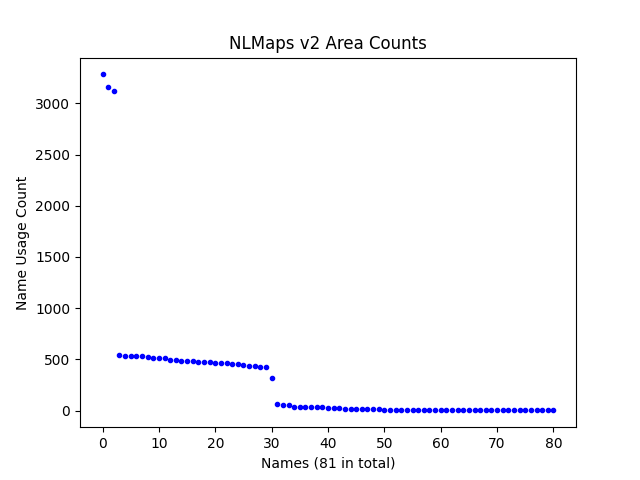
\includegraphics[width=\textwidth]{fig/nlmaps_v2_area_counts.png}
  \caption{Area values in \nlmapstwo{}}
  \label{fig:nlmaps-v2-areas}
\end{figure}

Some imbalance is also present in the values of \osmtag{name=*} tags in the
\mrl{nwr} operators, which are mostly names of points of interests. However, the
imbalance is much less pronounced in this case and with \num{5969} different
names there is a large variety of different names. This is illustrated in
Figure~\ref{fig:nlmaps-v2-nwrs}.

\begin{figure}[h]
  \centering
  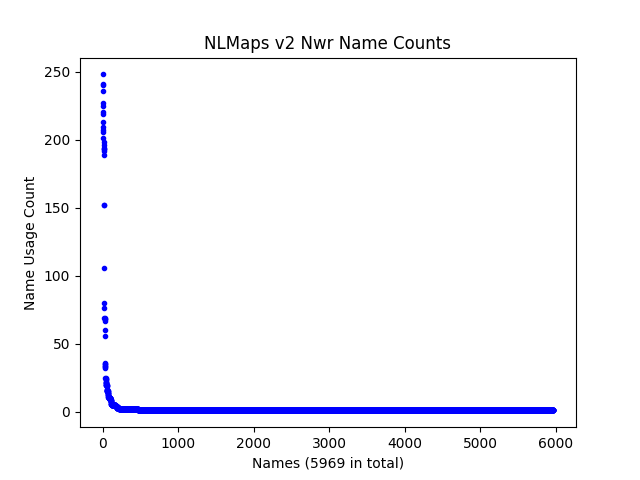
\includegraphics[width=\textwidth]{fig/nlmaps_v2_nwr_name_counts.png}
  \caption{Nwr values in \nlmapstwo{}}
  \label{fig:nlmaps-v2-nwrs}
\end{figure}

This lack of variety is not a problem when training on the masked data and using
an external NER system because the model will only ever see the placeholders for
the location names. However, models directly trained on \nlmapstwo{} will learn
a strong bias with respect to location names, as evidenced by the model
hallucinating the area \emph{Paris} out of thin air as seen in
Figure~\ref{fig:valleys-around-zenica}. An improved version of the dataset
should provide a large variety of names, which should also stem from a variety
of different countries and languages.

\subsection{Unnatural Wording of Queries}
\label{sec:unnatural-wording}

It is some queries’ purpose to extract the value associated with a certain key
from the result set, which is reflected in the MRL by operations like
\mrl{findkey('name')} or \mrl{findkey('opening_hours)} inside the \mrl{qtype}
clause. This intention can be coded in the NL query through wordings like
\nl{What are the names …?}, \nl{Name all the …!}, \nl{Tell me the
  opening hours …!} or \nl{When is … open?}.

This type of NL query is of course present in \nlmapstwo{}, but there are also
queries which are simply prefixed by an OSM key, which is then understood as an
indication to extract that key via the the \mrl{findkey} operator. Five such
queries are shown in Figure~\ref{fig:nlmaps-v2-unnatural-wording}. Some of them
(such as \nl{name Paris buy ice cream}) can pass as crude wordings of legitimate
queries.

\begin{figure}[h]
  \centering
  \begin{lstlisting}[basicstyle=\small]
wheelchair Jewelry Shops near München in walking distance
amenity closest Gas Station from Düsseldorf
bicycle Cycle Paths in Sheffield
source Sports Centres near Blakenhale Road in Birmingham
name Paris buy ice cream
  \end{lstlisting}
  \caption[Unnatural \nlmapstwo{} queries]{NL queries from \nlmapstwo{} where
    the OSM key that is to be extracted is just added as a prefix.}
  \label{fig:nlmaps-v2-unnatural-wording}
\end{figure}

Others are misleading or at least ambiguous. E.g., \nl{wheelchair Jewelry Shops
  near München in walking distance} is understood as being equivalent to
\nl{Tell me if the Jewelry Shops near München are wheelchair-accessible.},
whereas it could just as well mean \nl{Which Jewelry Shops near München are
  wheelchair-accessible?}, which might be the more likely query.

Some are actually nonsensical: Gas stations are selected via
\osmtag{amenity=fuel} in the first place, so the \osmtag{amenity} value will of
course always be \osmtag{fuel}; similarly for the bicycle path example. And some
keys are rarely worth asking for because they are in general not interesting,
such as the \osmtag{source} key, which is used by OSM mappers to give the
information source used for mapping an object (e.g. aerial photography or survey
in person).

Paired with the lack of linguistic variety, this method of unnaturally prefixing
an otherwise complete NL query with an OSM key is actually harmful when queries
are encountered that start with unseen phrases. This is evidenced by the query
\nl{Show me the cafes near Martinskirche in Westheim} in
Figure~\ref{fig:cafes-near-martinskirche}, where the model attempts to extract
the value of a nonsensical \osmtag{show:me} key.

With the exception of somewhat reasonable cases like prefixing \nl{name}, all of
these queries should be deleted from the dataset in order to improve it.

\subsection{Improper Usage of OSM Tags}
\label{sec:improper-osm-tags}

So far we have only discussed intrinsic qualities of \nlmapstwo{} by examining
NL and MRL queries and their consistency without paying heed to the usage of the
covered tags in the OSM database. This is of course important because the tags
only derive their meaning from their usage in the dataset. While most tags are
used correctly in \nlmapstwo{} (e.g. \osmtag{shop=clothes} used in MRLs for
queries asking for \nl{clothing stores}), there are also some tags that are not
in current use in OSM, have never been in use or their use differs from what
they are understood to mean in \nlmapstwo{}. Most of these errors are inherited
from the table discussed in Section~\ref{sec:term-tag-inconsistencies}. Some
examples are given:

\begin{itemize}
\item
  \osmtag{amenity=park}\footnote{\url{https://wiki.openstreetmap.org/wiki/Tag:amenity=park}.}
  is sometimes used in \nlmapstwo{}, even though \osmtag{leisure=park} is the
  proper tag for parks. As of April 2021, \osmtag{amenity=park} is used only
  \num{30} times in OSM.
\item \osmtag{place=house} has probably never had any usage in OSM, even though
  it is used in \nlmapstwo{}.
\item Churches\footnote{\url{https://wiki.openstreetmap.org/wiki/Church}.} are
  places of Christian worship and can be identified by the tag combination
  \osmtag{amenity=place_of_worship + religion=christian}. However, \nlmapstwo{}
  uses \osmtag{building=church} (and also \osmtag{historic=church}), which
  should be used for buildings \emph{built as} churches. They may be used for
  another purpose now\footnote{The Hagia Sophia mosque in Istanbul may be the
    most famous example of this.}, while some non-church buildings may be used
  for holding church services and are thus churches.\footnote{The analogous
    situation of a non-religious building being used as a mosque is very common
    in Germany, for example.}
\end{itemize}

Choosing the correct tag or tag combination is virtually irrelevant for training
the machine learning model, but it will obviously be essential when the MRLs are
actually used for an OSM lookup. Finer points of this multifaceted issue will be
discussed at a later point in this thesis.

\section{Improving on \nlmapstwo{}}

The most obvious way to produce a dataset that is closer to real world queries
is to source it from actual users via an annotation project. This is what will
be described later in this thesis. But in order to collect data efficiently, a
model is helpful that answers the simple questions correctly already, so that
annotators will spend less time constructing trivial MRLs. And even for more
difficult queries, it’s easier to adjust an MRL that is only slightly incorrect
than one with several errors.

Therefore, it is reasonable to make an effort of improving on the existing
\nlmapstwo{} dataset by fixing some of its shortcomings and by extending it with
new queries generated by an improved templating approach. These steps are
described in the following two sections.

\subsection{Fixing \nlmapstwo{} Shortcomings}

The fixing of shortcomings in the existing dataset concentrates on making it
more consistent. For reproducibility, all of the fixes are made in a
script,\footnote{\url{https://gitlab.cl.uni-heidelberg.de/will/nlmaps-tools/-/blob/handed_in/nlmaps_tools/fix_nlmaps_v2.py}.},
which does the following:

\begin{itemize}
\item OSM tags in the MRLs are replaced by non-deprecated counterparts or by the
  union of all applicable tags, in some cases depending on the content of the NL
  query. Cf. Sections~\ref{sec:term-tag-inconsistencies} and
  \ref{sec:improper-osm-tags}. Examples:
  \begin{itemize}
  \item \osmtag{amenity=park} \textrightarrow{} \osmtag{leisure=park}
  \item \osmtag{landuse=forest} \textrightarrow{} \mrl{or(landuse=forest,
      natural=wood)}
  \item NL asks for bars and MRL contains \osmtag{amenity=pub} \textrightarrow{}
    \osmtag{amenity=bar}
  \end{itemize}

\item The operator \mrl{area} in a \mrl{center} clause without an \mrl{nwr}
  operator is replaced by the \mrl{nwr} operator. Cf.
  Section~\ref{sec:mrl-inconsistencies}.

\item NL-MRL pairs where an OSM tag was used as the prefix of the NL query to
  indicate a matching \mrl{findkey} operator are removed with the exception of
  the keys \osmtag{name}, \osmtag{opening_hours} and \osmtag{website}. Cf.
  Section~\ref{sec:unnatural-wording}.
\end{itemize}

By applying these changes to \nlmapstwo{}, \num{2168} MRLs are modified and a
further \num{1859} instances are deleted resulting in a modified dataset
containing \num{26750} NL-MRL pairs, which will be called \nlmapstwoone{}. More
detailed numbers are given in Table~\ref{tab:nlmaps-v2.1-stats}. Note that the
NL side of queries is never modified in the process.

\begin{table}
  \centering
  \begin{tabular}{lrrrr}
    \toprule
    Split & \nlmapstwo{} & Modified & Deleted & \nlmapstwoone{}\\
    \midrule
    Train & \num{16172} & \num{1236} & \num{1059} & \num{15113}\\
    Dev & \num{1843} & \num{136} & \num{109} & \num{1734}\\
    Test & \num{10594} & \num{796} & \num{691} & \num{9903}\\
    \midrule
    Total & \num{28609} & \num{2168} & \num{1859} & \num{26750}\\
    \bottomrule
  \end{tabular}
  \caption[\nlmapstwoone{} statistics]{Numbers of deletions and modifications
    going from \nlmapstwo{} to \nlmapstwoone{}.}
  \label{tab:nlmaps-v2.1-stats}
\end{table}

\subsection{Extension of \nlmapstwo{}}

In order to address also the other shortcomings, a new dataset is generated in a
more sophisticated templating approach. The new approach differs by the one used
for \nlmapstwo{} in the following ways:

\begin{itemize}
\item More templates are used.
\item There is significant variation within each template.
\item More area names are used.
\item Area names are more evenly distributed.
\item More OSM tags are used. For this, the information from the table used for
  \nlmapstwo{} is manually extended.
\item Errors in the tag usage (as discussed in
  Sections~\ref{sec:term-tag-inconsistencies} and \ref{sec:improper-osm-tags})
  are of course avoided in the first place.
\end{itemize}

\begin{figure}[h]
  \centering
  \begin{lstlisting}[style=MyJinja]
when
{{ choose(['can I', 'can we', 'to'], [0.3, 0.3, 0.4]) }}
{{ choose(['visit', 'go to'], [0.6, 0.4]) }}

  {{ choose(['the', 'all', 'all the', ''], [0.2, 0.2, 0.2, 0.4]) }}

  {{ choose(['a', 'some', 'any', '']) }}

{{ thing_plural if plural else thing_singular }}

{{ optional('?') }}
  \end{lstlisting}
  \caption[Opening hours template]{Simple template for one version of queries
    for opening hours.}
  \label{fig:opening-hours-template}
\end{figure}

The templates are designed to be probabilistic. I.e., instead of being rigid,
they are essentially decision trees with various decisions being made to arrive
at the final wording of an NL query. Figure~\ref{fig:opening-hours-template}
shows one of several templates used for generating queries that ask for opening
hours. By choosing phrases according to the given probability distributions, it
can produce queries like \nl{when to visit theatres in Bratislava?} or \nl{when
  can I go to a cinema in Hannover}. The resulting dataet is called
\nlmapsthreea{}.

The location names are collected via extracting all areas and named places from
different regions in countries that use variations of the Latin alphabet. This
is done to ensure that location names from various languages are included in the
dataset.\footnote{When generating a query for things around some named place
  inside an area, both the place and the area are randomly selected
  independently from each other. This leads to queries like \nl{restaurants near
    Eiffel Tower in Rome}, which do not make sense in practice because there is
  no Eiffel Tower in Rome, but that doesn’t matter since the model is just
  supposed to learn to copy the names to the appropriate place in the MRL.}
Figure~\ref{fig:nlmaps-v3a-areas} shows a large variety in
well-distributed area names. This is in contrast with the situation in
\nlmapstwo{} shown in Figure~\ref{fig:nlmaps-v2-areas}.

\begin{figure}[h]
  \centering
  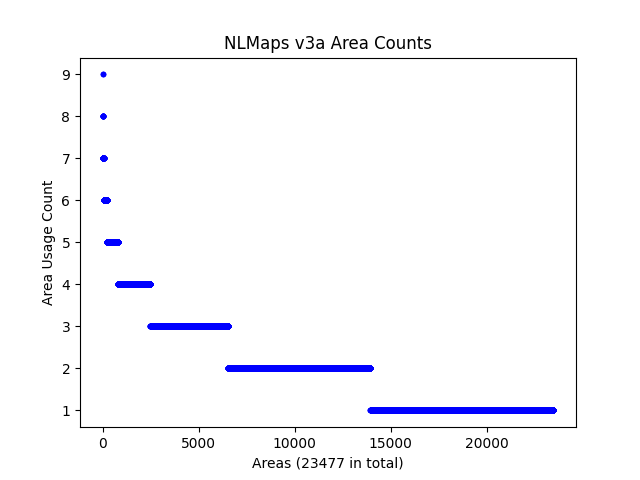
\includegraphics[width=\textwidth]{fig/nlmaps_v3a_area_counts.png}
  \caption{Area values in \nlmapsthreea{}}
  \label{fig:nlmaps-v3a-areas}
\end{figure}

In order to train models that are robust against typing errors and other small
spelling deviations, some noise is added to the NL queries in
\nlmapsthreea{} by switching a character for another with a chance of
\SI{1}{\%}. Names of locations are never touched, however. The resulting dataset
with noise is called \nlmapsthreeb{} and a random sample of NL queries is
shown in Figure~\ref{fig:nlmaps-v3b-sample}.

% TODO: The UTF-8 characters are messed up.
\begin{figure}[h]
  \centering
\begin{lstlisting}[style=MyNL]
what bathrooms in Záluží are around Zur Stöpe?
what preschools in Sadek are in walking distance hrom Gasthaus Tannengarten?
Do some veterinary surgerils exist east of studna in Montgeron (canton de Draveil)
Gire me any department store around ROBOT in Neue Vahr Südost
which setvice rosd in Bardzice is south of Le Ciré Jaune?
show me the opening times of all the monorail in the area of The KPH in Świecie
Which viewpoint is there in Miño de San Esteban?
In Grabowiec, what are the opening hours of all the boatyards less than 80 kilometres away from MakroMueble
Indicate the coordinaSes of all byways Tn přírodní památka Branžovy.
Are there parks east of Tigery?
\end{lstlisting}
  \caption[10 random \nlmapsthreeb{}.]{10 random \nlmapsthreeb{}.}
  \label{fig:nlmaps-v3b-sample}
\end{figure}

Finally, we concatenate \nlmapstwo{} and \nlmapsthreeb{} and call the result
\nlmapsthree{}. Since we generate exactly as many instances for
\nlmapsthreeb{} as are present in the corresponding split of \nlmapstwoone{},
\nlmapsthree{} is exactly twice as large as \nlmapstwoone{}.

The linguistic diversity of the resulting datasets is quantified by the entropy
rate estimated by the conditional entropy on trigrams, as described in
Section~\ref{sec:little-linguistic-diversity}. Table \ref{tab:v2-v3-overview}
offers an overview over the datasets.

\begin{table}[h]
  \centering
  \begin{tabular}{lrrrrr}
    \toprule
    Measure & \nlmtwo{} & \nlmtwoone{} & \nlmthreea{} & \nlmthreeb{} & \nlmthree{}\\
    \midrule
    Instances & \num{28609} & \num{26750} & \num{53500} & \num{53500} & \num{53500}\\
    Conditional Entropy & \num{2.11} & \num{2.08} & \num{2.85} & \num{2.93} & \num{2.73}\\
    Avg. Tokens per NL & \num{6.98} & \num{7.02} & \num{10.72} & \num{10.69} & \num{8.85}\\
    \bottomrule
  \end{tabular}
  \caption{Entropy rates estimated on trigrams.}
  \label{tab:v2-v3-overview}
\end{table}

%%% Local Variables:
%%% coding: utf-8
%%% mode: latex
%%% TeX-engine: xetex
%%% TeX-parse-self: t
%%% TeX-command-extra-options: "-shell-escape"
%%% TeX-master: "../thesis"
%%% End: